\section{Design}\label{sec: Design}
In this section the design and decisions that where made to achieve the laboratory are discussed.
%The code for lab 03 can be reviewed online under the flowing link \href{https://github.com/haringd/EGR680_FPGA_Labs/tree/master/VENDMACH}{http://github.com/haringd/EGR680\_FPGA\_Labs/tree/master/VENDMACH}.
\subsection{Lab specification}\label{subsec: Lab specification}
In this part,a simple program in C is developed that takes the user input of two dip switches and represents it in binary on the on board LEDs. The user input is printed out over UART terminal as well as the user input of the buttons. 

The binary user input of the dip switches is passed into the hardware instantiated decoder which is implemented in an user created IP module. The module consist out of an 7 bit output for one seven-segment display and the carry bit, which is used to switch between the two segments.
The diagram for the partial design is shown in Figure \ref{fig: Vivado_lab4_CompletedDesign}. The designed seven\_seg\_ip is connected over the AXI bus like the LED\_IP. 
\begin{figure}[H]
	\centering
	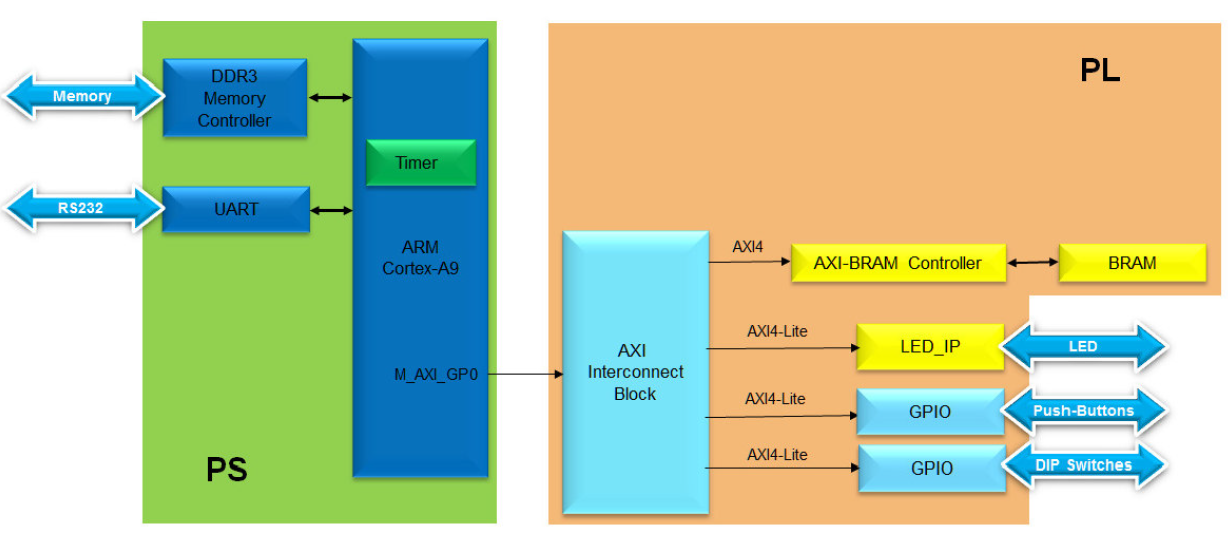
\includegraphics[width=1.0\textwidth]{01_images/Vivado_lab4_CompletedDesign.PNG}
	\caption{Completed Design.}
	\label{fig: Vivado_lab4_CompletedDesign}
\end{figure}

\subsection{HDL}\label{subsec: HDL}
Figure \ref{fig: Vivado_lab_HDL_topView} shows the HDL top level based of the ZYNQ 7 Processing system which is connected with an AXI bus S\_AXI to a intellectual property (IP) block that manages peripherals. From there an AXI bus is used to connect two general purpose input output (GPIO) IP blocks, one for buttons and another one for switches. Furthermore, a Processor System Reset IP block is used that interconnects all resets. The block of interest is the added seven\_seg\_ip that is used to decode the user input into the seven-segment display.
\begin{figure}[H]
	\centering
	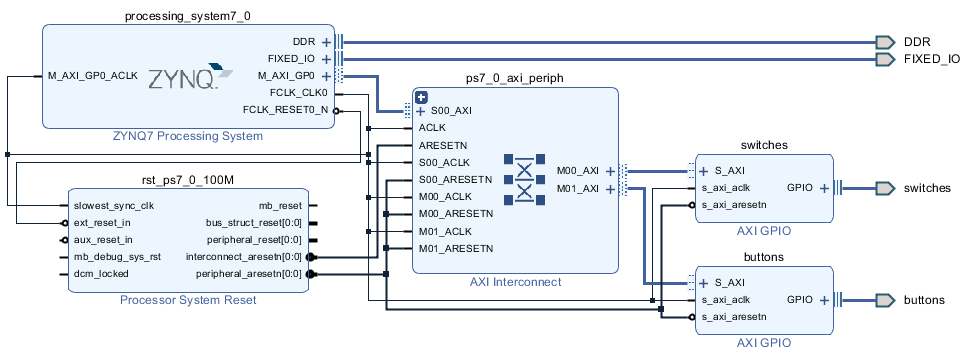
\includegraphics[width=1.0\textwidth]{01_images/Vivado_lab_HDL_topView.PNG}
	\caption{HDL Top Level Design.}
	\label{fig: Vivado_lab_HDL_topView}
\end{figure}

\subsection{SDK}\label{subsec: SDK}
After the HDL top level is defined the SDK can be launched with \textbf{File $\rightarrow$ Launch SDK}. The *.hdf file should be shown or can be opened that shows the base registers for the switches, led, seven-segment display, and buttons, as shown in Figure \ref{fig: Vivado_lab4_SW_BTN_Register}. 
\begin{figure}[H]
	\centering
	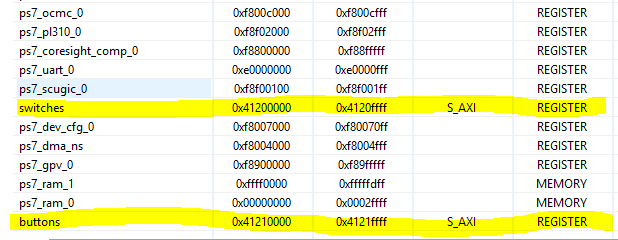
\includegraphics[width=1.0\textwidth]{01_images/Vivado_lab4_SW_BTN_Register.PNG}
	\caption{*.hdf file that shows the base register for switches, led, seven-segment display, and buttons.}
	\label{fig: Vivado_lab5_SW_BTN_Register}
\end{figure}

After writing the C code the FPGA bit stream file and the build elf file can be loaded onto the board. The serial console Terra Term shows the status of the buttons and switches, as shown in Figure \ref{fig: Vivado_lab4_TT_PartII}. The C code could basically used entyrely from the former lab and only the lines 17 and 40 had to be added.
\begin{figure}[H]
	\centering
	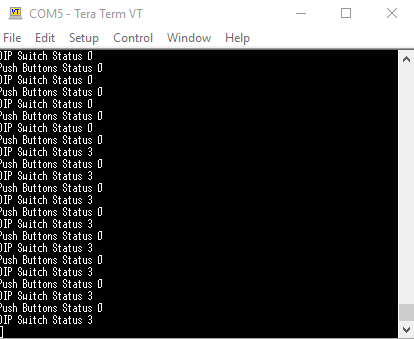
\includegraphics[width=0.7\textwidth]{01_images/Vivado_lab4_TT_PartII.PNG}
	\caption{Terra Term print out of the switches and buttons status.}
	\label{fig: Vivado_lab4_TT_PartII}
\end{figure}

